% 架构图 - 使用TikZ绘制
% 在main.tex中添加 \usepackage{tikz} 后可直接使用

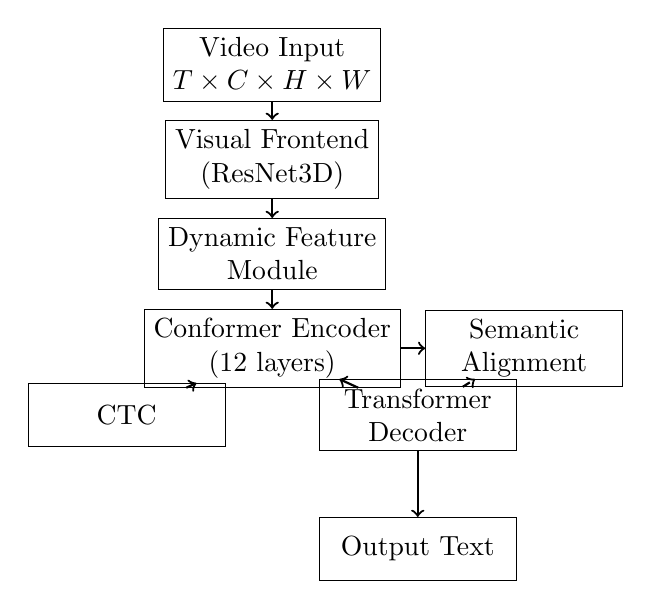
\begin{tikzpicture}[
    node distance=1.2cm,
    box/.style={rectangle, draw, minimum width=2.5cm, minimum height=0.8cm, align=center},
    arrow/.style={->, thick}
]

% 输入
\node[box] (input) {Video Input\\$T \times C \times H \times W$};

% Visual Frontend
\node[box, below of=input] (frontend) {Visual Frontend\\(ResNet3D)};

% Dynamic Feature Module
\node[box, below of=frontend] (dynamic) {Dynamic Feature\\Module};

% Conformer Encoder
\node[box, below of=dynamic] (encoder) {Conformer Encoder\\(12 layers)};

% 分支
\node[box, below left of=encoder, xshift=-1cm] (ctc) {CTC};
\node[box, below right of=encoder, xshift=1cm] (decoder) {Transformer\\Decoder};

% Semantic Alignment
\node[box, right of=encoder, xshift=2cm] (align) {Semantic\\Alignment};

% 输出
\node[box, below of=decoder, yshift=-0.5cm] (output) {Output Text};

% 连接
\draw[arrow] (input) -- (frontend);
\draw[arrow] (frontend) -- (dynamic);
\draw[arrow] (dynamic) -- (encoder);
\draw[arrow] (encoder) -- (ctc);
\draw[arrow] (encoder) -- (decoder);
\draw[arrow] (encoder) -- (align);
\draw[arrow] (decoder) -- (output);
\draw[arrow, dashed] (align) -- (decoder);

\end{tikzpicture}
